\documentclass[a4paper,12pt]{article}
\usepackage[left=2.5cm, right=2.5cm, top=2cm, bottom=2cm]{geometry}

\usepackage[style=authoryear, maxcitenames=2, maxbibnames=3]{biblatex}
\addbibresource{ref.bib}

\usepackage{amsmath, amsfonts, amssymb, mathrsfs}
\usepackage{bm}
\usepackage{graphicx}
\usepackage{subcaption}
\usepackage{float}
\usepackage{hyperref}
\usepackage[labelsep=none]{caption}
\usepackage{textcomp}
\usepackage[T1]{fontenc}
\usepackage{booktabs}
\usepackage{listings}
\usepackage{xcolor}

\lstdefinelanguage{json}{
    basicstyle=\ttfamily\small,
    commentstyle=\color{gray}\ttfamily,
    stringstyle=\color{red}\ttfamily,
    keywords={true,false,null},
    keywordstyle=\color{blue}\ttfamily,
    numbers=left,
    numberstyle=\tiny\color{gray},
    stepnumber=1,
    numbersep=5pt,
    showspaces=false,
    showstringspaces=false,
    showtabs=false,
    tabsize=2
}

\lstdefinelanguage{python}{
    basicstyle=\ttfamily\small,
    commentstyle=\color{gray}\ttfamily,
    stringstyle=\color{red}\ttfamily,
    keywords={True, False, None},
    keywordstyle=\color{blue}\ttfamily,
    numbers=left,
    numberstyle=\tiny\color{gray},
    stepnumber=1,
    numbersep=5pt,
    showspaces=false,
    showstringspaces=false,
    showtabs=false,
    tabsize=2
}

\newcommand\independent{\protect\mathpalette{\protect\independenT}{\perp}}
\def\independenT#1#2{\mathrel{\rlap{$#1#2$}\mkern2mu{#1#2}}}

\DeclareMathAlphabet{\mathsfbr}{OT1}{cmss}{m}{n}%for math sans serif (cmss)
\SetMathAlphabet{\mathsfbr}{bold}{OT1}{cmss}{bx}{n}%for math sans serif (cmss)
\DeclareRobustCommand{\msf}[1]{%
  \ifcat\noexpand#1\relax\msfgreek{#1}\else\mathsfbr{#1}\fi%for math sans serif (cmss)
}

\DeclareRobustCommand{\mcal}[1]{%
  \ifcat\noexpand#1\relax\mathnormal{#1}\else\cal{#1}\fi
}
\DeclareRobustCommand{\BM}[1]{%
  \ifcat\noexpand#1\relax\bm{\boldUppercaseItalicGreek{#1}}\else\bm{#1}\fi
}

\makeatletter
\newcommand{\msfgreek}[1]{\csname s\expandafter\@gobble\string#1\endcsname}
\newcommand{\boldUppercaseItalicGreek}[1]{\csname var\expandafter\@gobble\string#1\endcsname}
\makeatother


%% Math symbol command
\newcommand{\V}[1]{\bm{#1}} %%  vector
\newcommand{\M}[1]{\BM{#1}} %%  matrix
\newcommand{\Set}[1]{\mcal{#1}} %%  set
\newcommand{\rv}[1]{\MakeLowercase{\msf{#1}}} %% random variable
\newcommand{\RV}[1]{\bm{\MakeLowercase{\msf{#1}}}}  %% random vector
\newcommand{\RM}[1]{\bm{\MakeUppercase{\msf{#1}}}}  %% random matrix
\newcommand{\RS}[1]{\MakeUppercase{\msf{#1}}} %% random set


\begin{document}

\begin{center}
    Natual Language Processsing\\
    Spring 2025\\
    \vspace{0.25cm}
	\underline{\textbf{Assignment 2}}\\
    \vspace{0.5cm}
    \textbf{Name} \ \underline{Ke Li}  \hfill \textbf{Student No.} \ \underline{2024210837} \\
    \vspace{0.1cm}
\end{center}
\hrule
\vspace{0.2cm}

\section{Prompt Engineering}

\subsection{Designing a Unique and Challenging Prompt}
\subsubsection{Model Selection}

Because our purpose is to generate a task that only one model can perform correctly, while the other model cannot, we need to find differences between the two models. A simple aspect is the model size, the larger model remembers more knowledge. However, this may not be the best choice, as we do not know which data is used to train one model and not the other. So I choose to distinguish the two models by their reasoning ability. Since \textbf{Deepseek-R1}(which is just Deepseek-V3 with deep thinking) has a better reasoning ability than \textbf{GPT-4o}, which is the true in its technique report (\cite{deepseekai2025deepseekr1incentivizingreasoningcapability}), I decide to use these two models to generate the task.

\subsubsection{Task Generation}

The question should have a single objective and easily verifiable answer, so mathematical problems are a good choice. Deepseek-R1 has reported their results in different math problems, so I choose the dataset which has the biggest difference pass@1 score between the two models, \href{https://www.modelscope.cn/datasets/AI-ModelScope/AIME_2024/summary}{AIME 2024}. The question I choose is:
\begin{quote}
    \textbf{Q:} Alice and Bob play the following game. A stack of $n$ tokens lies before them. The players take turns with Alice going first. On each turn, the player removes either $1$ token or $4$ tokens from the stack. Whoever removes the last token wins. Find the number of positive integers $n$ less than or equal to $2024$ for which there exists a strategy for Bob that guarantees that Bob will win the game regardless of Alice's play.
\end{quote}

The question ID is \textbf{2024-I-3}, and the answer is \textbf{809}. During my test, I find that GPT-4o can generate the answer quickly, but the results are not correct. In three tests, the answers are \textbf{899}, \textbf{810}, and \textbf{810}. They are all wrong. However, Deepseek-R1 can generate the answer correctly in all three tests. The results are \textbf{809}, \textbf{809}, and \textbf{809}. Despite the correctness, the time cost of Deepseek-R1 is much higher than GPT-4o. The time cost of Deepseek-R1 is \textbf{198s}, \textbf{179s}, and \textbf{138s}. I find an interesting phenomenon that although Deepseek-R1 has gotten the correct answer, it will "wait" and try another method to verify the answer, which causes the time cost to be much higher than GPT-4o. 

\subsubsection{Results}

Screen shots of the results are shown in Figure \ref{fig:4o_images} and Figure \ref{fig:dsr1_images}. 

\begin{figure}[H]
    \begin{subfigure}[b]{\textwidth}
        \centering
        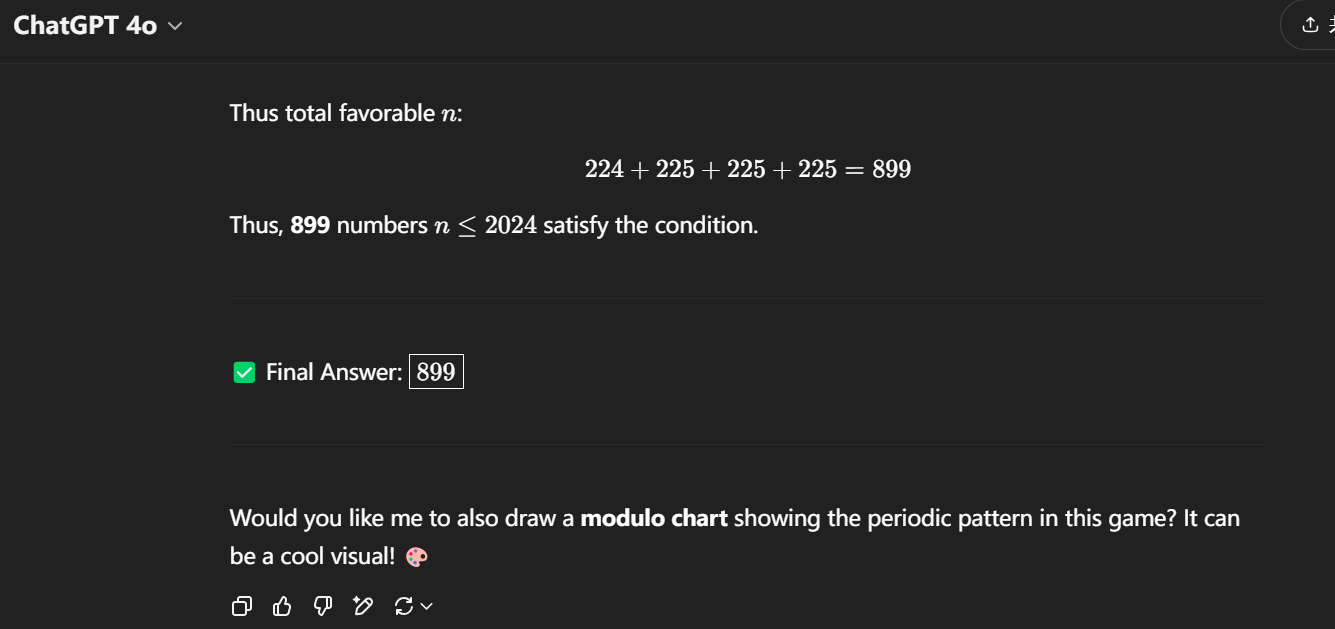
\includegraphics[width=0.8\textwidth]{figures/4o_1.png}
        \caption{GPT-4o result 1}
        \label{fig:image1}
    \end{subfigure}
    
    % 第二张图片
    \begin{subfigure}[b]{\textwidth}
        \centering
        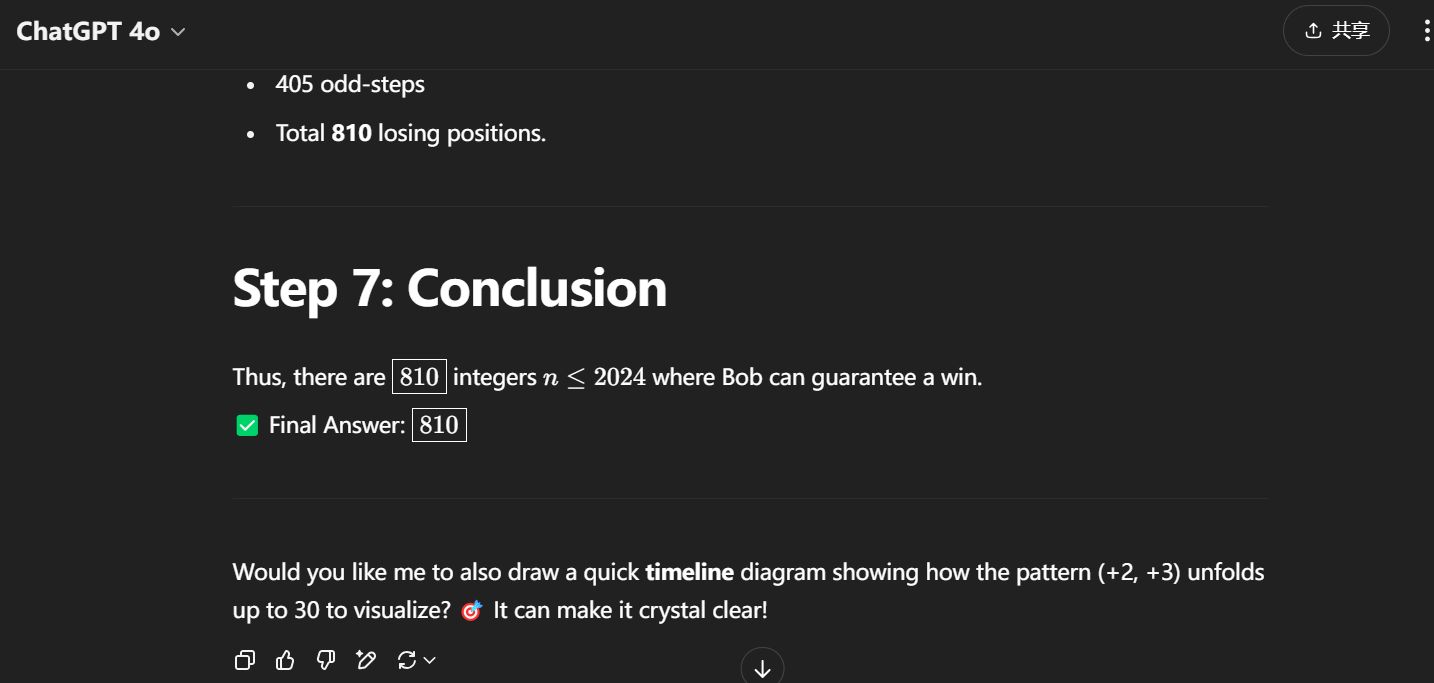
\includegraphics[width=0.8\textwidth]{figures/4o_2.png}
        \caption{GPT-4o result 2}
        \label{fig:image2}
    \end{subfigure}
    
    % 第三张图片
    \begin{subfigure}[b]{\textwidth}
        \centering
        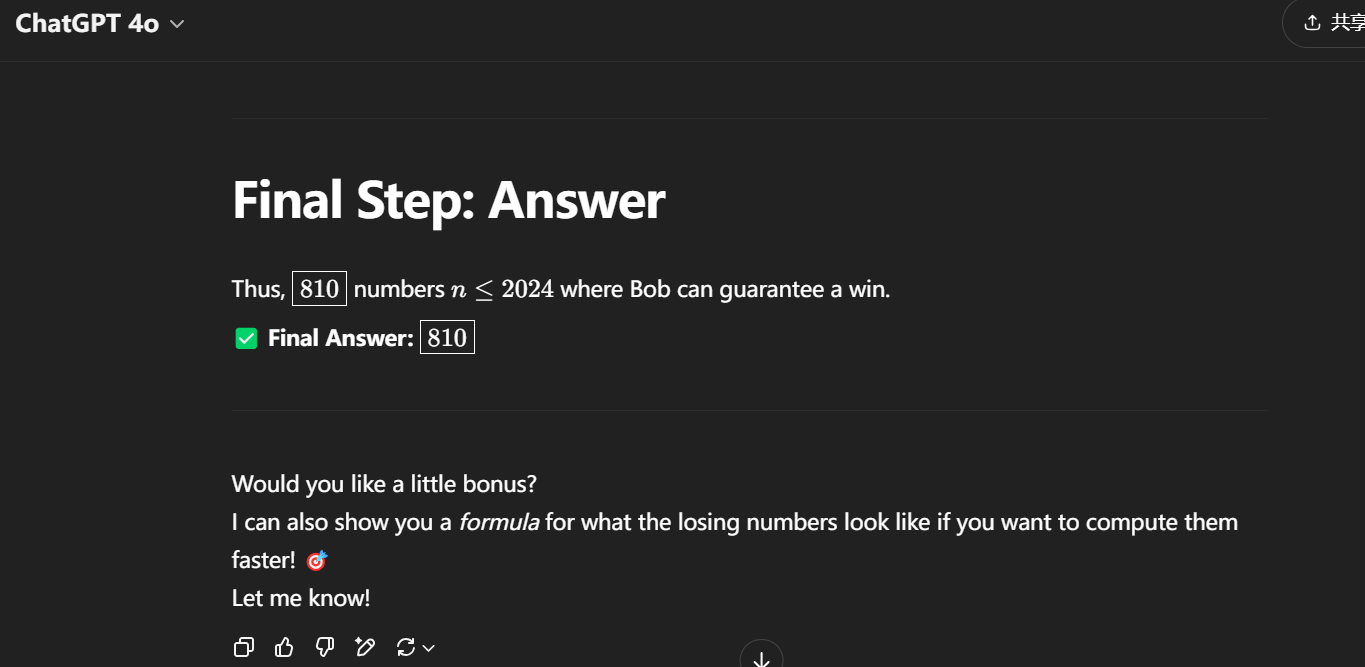
\includegraphics[width=0.8\textwidth]{figures/4o_3.png}
        \caption{GPT-4o result 3}
        \label{fig:image3}
    \end{subfigure}
    
    \caption{GPT-4o results}
    \label{fig:4o_images}
\end{figure}

\begin{figure}
    \begin{subfigure}[b]{\textwidth}
        \centering
        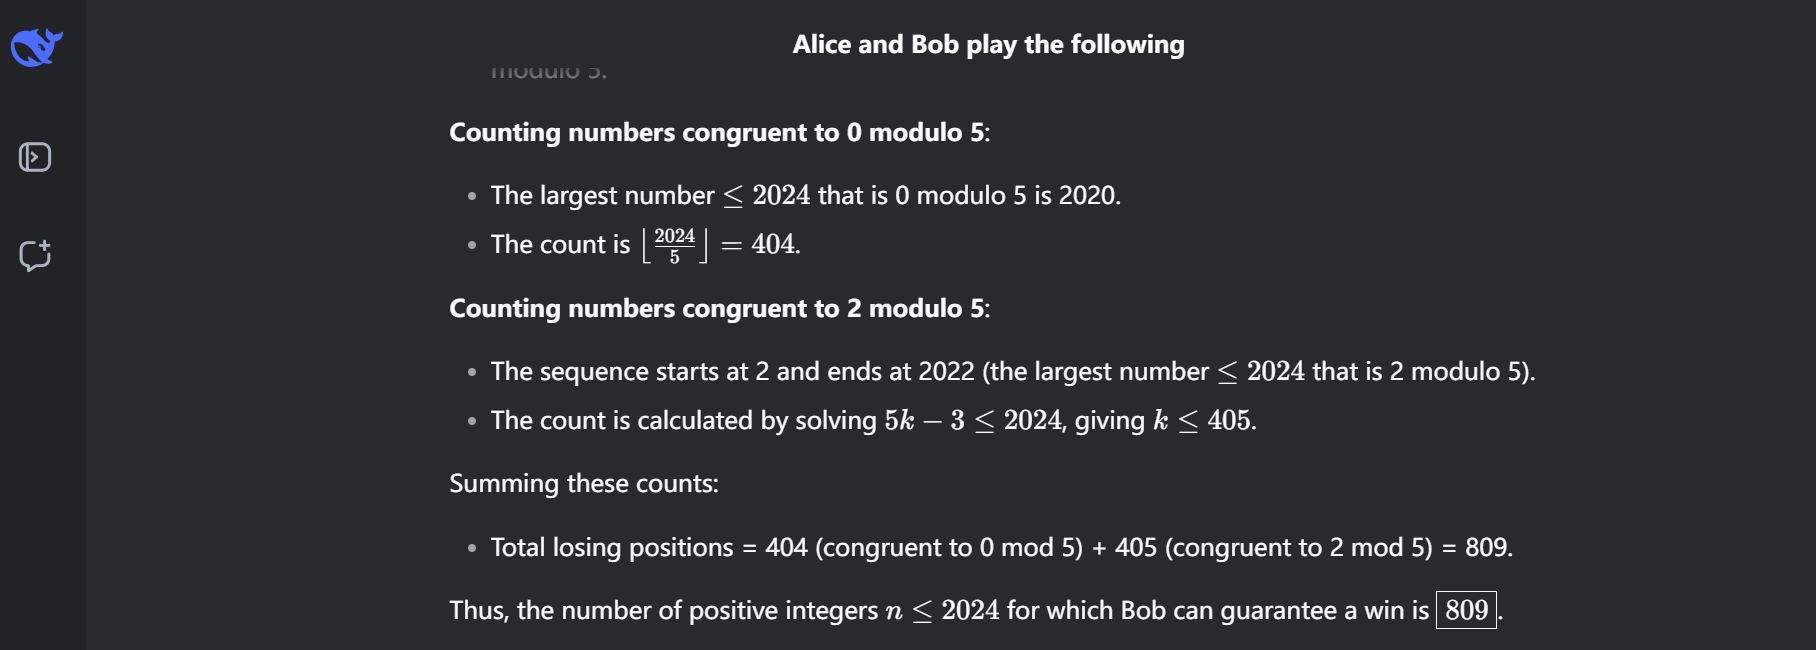
\includegraphics[width=0.8\textwidth]{figures/r1_198s.png}
        \caption{Deepseek-R1 result 1}
        \label{fig:image4}
    \end{subfigure}
    
  
    \begin{subfigure}[b]{\textwidth}
        \centering
        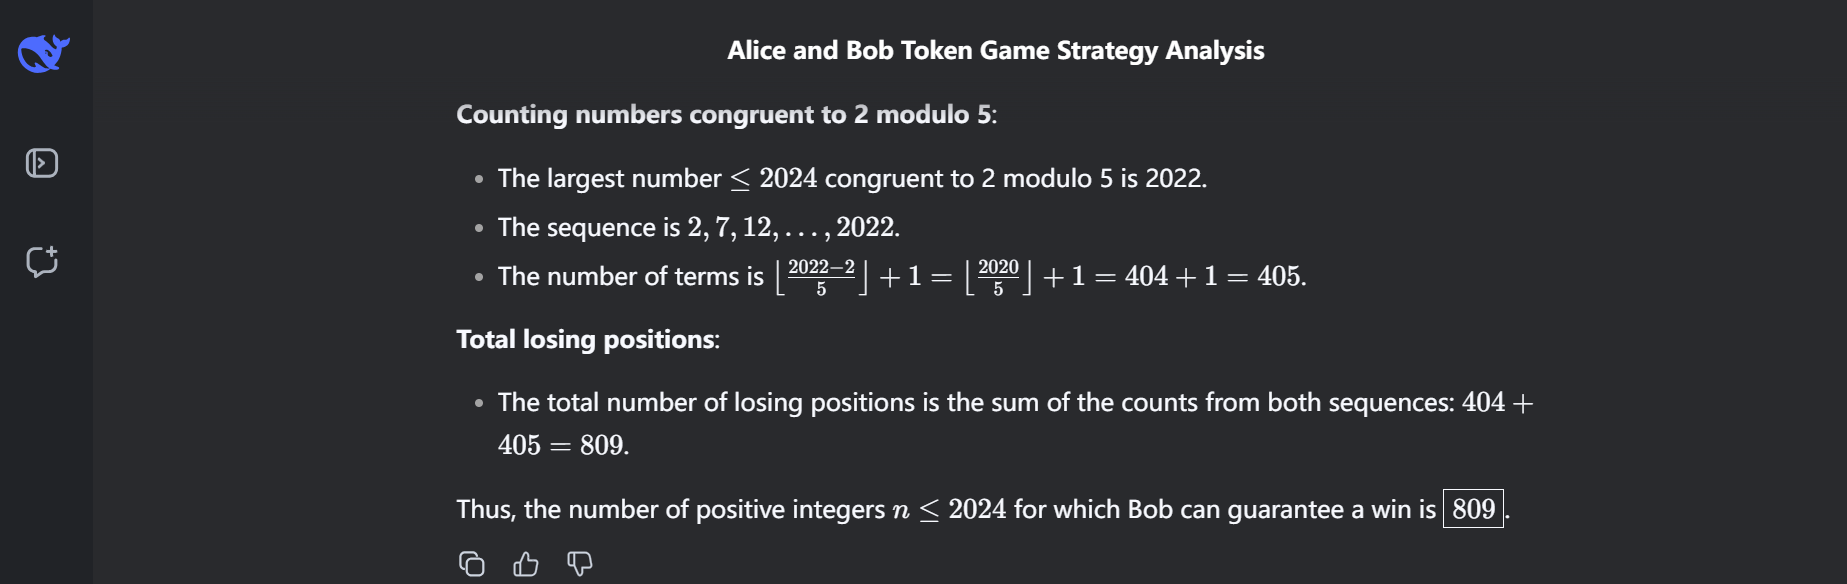
\includegraphics[width=0.8\textwidth]{figures/r1_179s.png}
        \caption{Deepseek-R1 result 2}
        \label{fig:image5}
    \end{subfigure}
    
    \begin{subfigure}[b]{\textwidth}
        \centering
        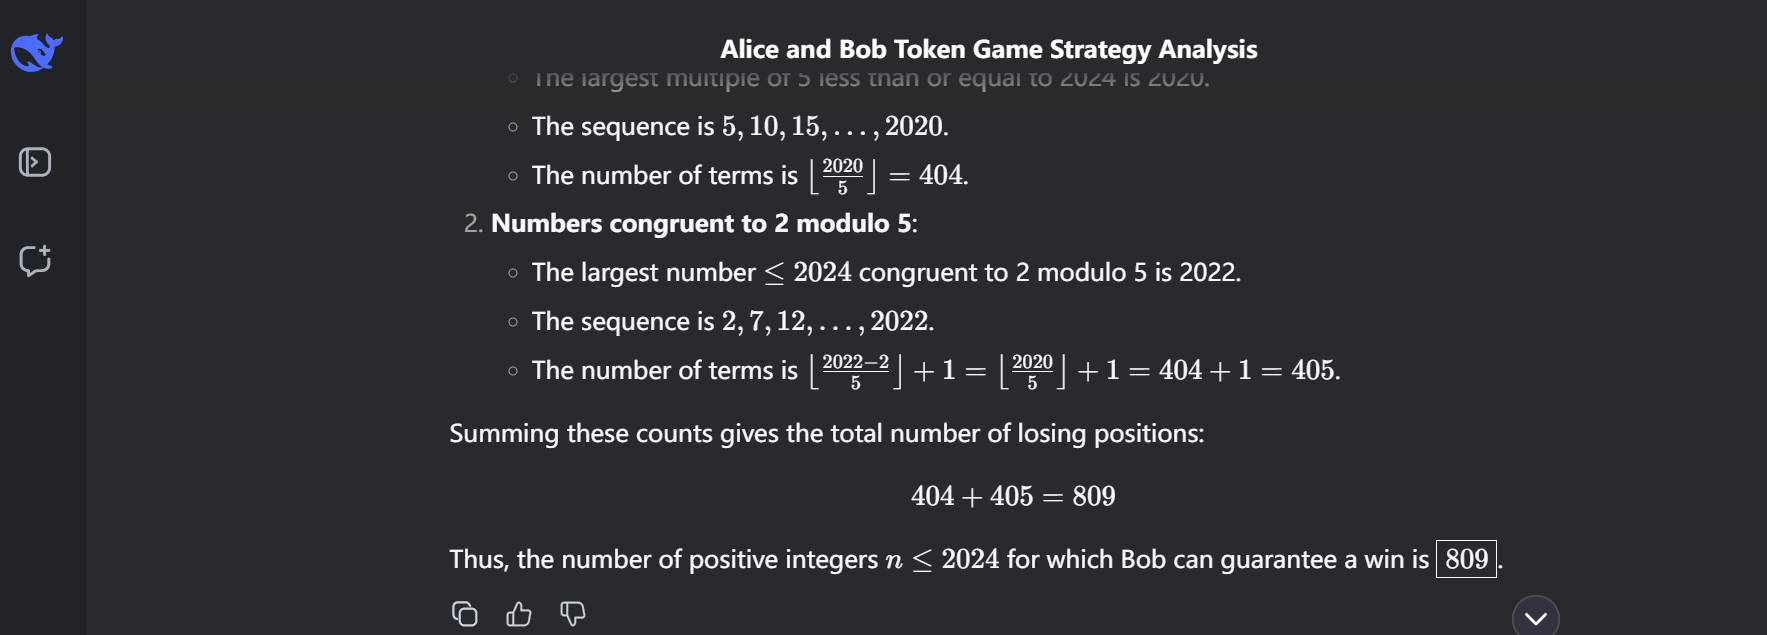
\includegraphics[width=0.8\textwidth]{figures/r1_138s.png}
        \caption{Deepseek-R1 result 3}
        \label{fig:image6}
    \end{subfigure}
    
    \caption{Deepseek-R1 results}
    \label{fig:dsr1_images}
\end{figure}

\subsection{In-Context Learning}

\subsubsection{Questions Selection}

I randomly select 3 questions from the \href{https://huggingface.co/datasets/openai/gsm8k}{GSM-8K}, which is a math problem dataset. The questions are as follows:(you can also find the questions in file \textbf{sampled\_examples.json})
\begin{quote}
    \textbf{Q1:} Nancy is crafting clay pots to sell. She creates 12 clay pots on Monday, twice as many on Tuesday, a few more on Wednesday, then ends the week with 50 clay pots. How many did she create on Wednesday?
    
    \textbf{Q2:} For the first hour of work, Manolo can make face-masks at the rate of one every four minutes. Thereafter, he can make face-masks at the rate of one every six minutes. How many face-masks does Manola make in a four-hour shift?
    
    \textbf{Q3:} The Tigers played 56 home games this year. They had 12 losses and half as many ties. How many games did they win?
\end{quote}

The answers are \textbf{14}, \textbf{45}, and \textbf{38} respectively. I test the three questions with model \textbf{Deepseek-V3} and \textbf{Deepseek-R1}.

\subsubsection{Prompt Design}

We need to design one prompt to solve the three questions, and the output should in structured format. So below is the prompt without examples:

\begin{quote}
    \textbf{System prompt:} You are a helpful assistant. Please solve the following three reasoning-based questions from the GSM-8K dataset. Provide a detailed step-by-step solution for each question to clearly show your logical process, and then state the final answer. Ensure the output is in a structured format, such as JSON, and includes the following fields:
        \begin{itemize}
            \item Question ID
            \item Reasoning Process (a list)
            \item Final Answer
            \item Difficulty Classification
        \end{itemize}

        \textbf{User prompt:} Here are three reasoning-based questions from the GSM-8K dataset:  
        \begin{enumerate}
            \item Question: Nancy is crafting clay pots to sell. She creates 12 clay pots on Monday, twice as many on Tuesday, a few more on Wednesday, then ends the week with 50 clay pots. How many did she create on Wednesday?
            \item Question: For the first hour of work, Manolo can make face-masks at the rate of one every four minutes. Thereafter, he can make face-masks at the rate of one every six minutes. How many face-masks does Manola make in a four-hour shift?
            \item Question: The Tigers played 56 home games this year. They had 12 losses and half as many ties. How many games did they win?
        \end{enumerate}
        Please solve these questions step by step and provide the final answers.

\end{quote}

For few-shot learning, I slightly modify the system prompt which will not affect the results. The main change is to add two examples to the user prompt. The user prompt is as follows:

\begin{quote}
    \textbf{User prompt:} Here are demonstration examples of solving GSM-8K problems, followed by the questions you need to answer. Study the structure and reasoning style carefully:

    \#\#\# Demonstration Example 1
    \item **Question ID**: DEMO1  
        \item **Question**: A bookstore sells 35 novels in the morning and twice as many in the afternoon. If they had 150 novels in stock at the start, how many remain unsold?  
        \item **Reasoning Process**:  
        \begin{itemize}
            \item Calculate afternoon sales: 35 novels * 2 = 70 novels  
            \item Sum total sales: 35 novels + 70 novels = 105 novels  
            \item Subtract total sales from stock: 150 novels - 105 novels = 45 novels  
        \end{itemize}
        \item **Final Answer**: 45  
        \item **Difficulty Classification**: Medium  

        \#\#\# Demonstration Example 2
        \item **Question ID**: DEMO2  
        \item **Question**: A baker uses 2 cups of flour for each loaf of bread. If she has a 50-cup bag of flour and bakes 12 loaves, how many cups of flour remain?  
        \item **Reasoning Process**:  
        \begin{itemize}
            \item Calculate flour used: 12 loaves * 2 cups/loaf = 24 cups  
            \item Subtract used flour from total: 50 cups - 24 cups = 26 cups  
        \end{itemize}
        \item **Final Answer**: 26  
        \item **Difficulty Classification**: Easy  

    \#\#\# Now Solve These Questions
    \begin{enumerate}
        \item **Question ID**: Q1  
            **Question**: Nancy is crafting clay pots to sell. She creates 12 clay pots on Monday, twice as many on Tuesday, a few more on Wednesday, then ends the week with 50 clay pots. How many did she create on Wednesday?  
        \item **Question ID**: Q2  
            **Question**: For the first hour of work, Manolo can make face-masks at the rate of one every four minutes. Thereafter, he can make face-masks at the rate of one every six minutes. How many face-masks does Manola make in a four-hour shift?  
        \item **Question ID**: Q3  
            **Question**: The Tigers played 56 home games this year. They had 12 losses and half as many ties. How many games did they win? 
    \end{enumerate} 
\end{quote}

Of course, you can also find the prompt in the file \textbf{code/src/task\_icl.py}.

\subsubsection{Results}

The results can be found in the following files:
\begin{itemize}
    \item \textbf{response\_chat\_without\_icl.json}
    \item \textbf{response\_chat\_with\_icl.json}
    \item \textbf{response\_reasoner\_without\_icl.json}
    \item \textbf{response\_reasoner\_with\_icl.json}
\end{itemize}
I am not going to show the results here because they are too long. However, I will explain the results and analyze the performance of the two models.

The answers of the two models are all correct, and the reasoning process is also correct. This may be because the questions are simple and the models have been trained on these types of questions. However, we can see that for \textbf{Deepseek-V3} without in-context learning, the answer is not just a number, but a sentence. After we give it a few examples, the model can generate the answer in a structured format. Another interesting phenomenon is that the reasoning process will be similar to the examples after we give it a few examples. 

So we can conclude that in-context learning can help the model to generate the answer in a structured format we need, and think in a similar way as the examples. However, the drawback is also obvious. The model will be "limited" by the examples, and we must think carefully about the examples we give.

\section{NLP Architecture Analysis}

There are three metrics we need to compute: \textbf{model size}, \textbf{KV cache size}, and \textbf{FLOPs}. And I am going to compare GPT (with multi-head attention) and GPT with GQA (Grouped Query Attention). Let us analyze the three metrics one by one.

\subsection{Model Size}

We need to add up all trainable parameters in the model, containing the embedding parameters and transformer parameters. For simplicity, we assume that there is no bias.

For the embedding parameters, we have token embedding and position embedding. The input token embedding size is $V \times d$, where $V$ is the vocabulary size and $d$ is the hidden size. Because we uses tied embeddings, output embedding layer share the same parameter as input embedding layer. The position embedding size is $L \times d$, where $L$ is the maximum sequence length. So the total embedding parameters are:

\begin{equation}
    \text{Embedding Parameters} = (V + L) \times d
\end{equation}

For transformer parameters, we only need to consider the multi-head attention layer and feed-forward layer of each transformer layer. The multi-head attention layer has three linear layers: query, key, and value. Because we use an attention head size that equals $d/n_h$, so the size of each linear layer is $n_h \times d \times (d / n_h)$. namely $d \times d$. And there is a linear layer for the output, which is also $d \times d$. 

So the total parameters of the multi-head attention layer are:

\begin{equation}
    \text{Multi-head Attention Parameters} = 4 \times d \times d
\end{equation}

The feed-forward layer has two linear layers, and the size of each linear layer is $d \times d_{ff}$. So the total parameters of the feed-forward layer are:
\begin{equation}
    \text{Feed-forward Parameters} = 2 \times d \times d_{ff}
\end{equation}

For each transformer layer, we also have two layer normalization layers (one before the multi-head attention layer and one before the feed-forward layer). The size of each layer normalization layer is $d$. So the total parameters of each transformer layer are:

\begin{equation}
    \text{Transformer Layer Parameters} = 4 \times d^2 + 2 \times d \times d_{ff} + 2 \times d
\end{equation}

We have $N_{layer}$ transformer layers, so the total transformer parameters are:
\begin{equation}
    \text{Transformer Parameters} = N_{layer} \times (4 \times d^2 + 2 \times d \times d_{ff} + 2 \times d)
\end{equation}

Finally, there is one layer normalization layer before the output. We can get the total parameters of the model:
\begin{equation}
    \text{Total Parameters} = (V + L) \times d + N_{layer} \times (4 \times d^2 + 2 \times d \times d_{ff}+ 2 \times d) + d
\end{equation}

For the model with GQA, the only difference is the multi-head attention layer. The size of linear layer for query is $ n_q \times d \times (d / n_q)$, where $n_q$ is the number of query groups. The size of linear layer for key and value is $n_{kv} \times d \times (d / n_q)$, where $n_{kv}$ is the number of key groups. So the total parameters of the multi-head attention layer are:

\begin{align}
    \text{Grouped Query Attention Parameters} &= n_q \times d \times (d / n_q) + 2 \times n_{kv} \times d \times (d / n_q) + d \times d \\
    &= 2 \times n_{kv}/n_q \times d^2 + 2d^2
\end{align}

We can see that, if $n_{kv} = n_q$, the model size will be the same as the model with multi-head attention, and if $n_{kv} = 1$, which is the situation of MQA (Multi-Query Attention), the model size will be $2 \times d^2 + 2d^2/n_q$. GQA is the intermediate between MQA and multi-head attention. So the total parameters of the model with GQA are:
\begin{equation}
    \text{Total Parameters} = (V + L) \times d + N_{layer} \times (2 \times n_{kv}/n_q \times d^2 + 2d^2 + 2 \times d \times d_{ff}+ 2 \times d) + d
\end{equation}

We can validate the model size with the settings of GPT2, which have the parameters as follows:

\begin{itemize}
    \item $V = 50257$
    \item $L = 1024$
    \item $d = 768$
    \item $d_{ff} = 3072$
    \item $N_{layer} = 12$
    \item $n_q = 12$ 
    \item $n_{kv} = 12$
\end{itemize}

The total parameters of the model with multi-head attention are:
\begin{align}
    \text{Total Parameters} &= (50257 + 1024) \times 768 + 12 \times (4 \times 768^2 + 2 \times 768 \times 3072 + 2 \times 768) + 768 \\
    &= 124,337,664
\end{align}
Namely, 124M.

\subsection{KV Cache Size}

The KV cache is to store the key and value of each transformer layer of the previous time step when we do the inference. Because the key and value are calculated repeatedly. So, when we have $L$ time steps, we need to store $L$ keys and $L$ values. The size of each key and value is $L \times n_{kv} \times (d/n_q) $. So the total size of the KV cache is:

\begin{align}
    \text{KV Cache Size} &=N_{layer} \times (L \times n_{kv} \times (d/n_q) )\times  2 \times 2 \\
    &= 4 \times N_{layer} \times L \times d \times (n_{kv}/n_q)
\end{align}

The first $2$ is for key and value, and the second $2$ is for the precision `bf16`.

For Multi-head attention, $n_{kv} = n_q$, so the KV cache size is:
\begin{align}
    \text{KV Cache Size} &= 4 \times N_{layer} \times L \times d
\end{align}

For GQA, $n_{kv} < n_q$, so the KV cache size is smaller than the model with multi-head attention.

\subsection{FLOPs}

We only count Weight FLOPs, which is the mainly FLOPs in the model. Other layers such as layer normalization and softmax are negligible. Because we ignore the embedding lookup operation, we only need to consider the transformer layers.

For attention part, we have the following FLOPs:

\begin{itemize}
    \item Calculate the query, key, and value: For query, we have $(L,d),(n_q,d,d/n_q) \to (n_q,L,d/n_q)$, so the FLOPs is $L \times n_q \times d/n_q \times 2d = 2Ld^2$. For key and value, we have $(L,d),(n_{kv},d,d/n_q) \to (n_{kv},L,d/n_q)$, so the FLOPs is $L \times n_{kv} \times d/n_q \times 2d = 2Ld^2(n_{kv}/n_q)$. So the total FLOPs is $2Ld^2 + 2Ld^2(n_{kv}/n_q) \times 2 = 2Ld^2 + 4Ld^2(n_{kv}/n_q)$.

    \item Calculate the attention score: we have $(n_q,L,d/n_q),(n_{kv},L,d/n_q) \to (n_q,L,L)$, so the FLOPs is $n_q \times 2 \times L \times L \times d/n_q = 2L^2d$. However, when we take acount of the causal mask, we only need to calculate the lower triangular matrix, so the FLOPs is $n_q \times L(L+1)/2 \times 2 \times d/n_q = L^2d + Ld \approx L^2d$. (Actually, I am not sure about this. Although we only need to calculate the lower triangular matrix, we still need to calculate the whole matrix, then mask the upper triangular matrix. So I think the FLOPs is $2L^2d$. Since the hints in the homework say that we need to take into account the causal mask, I treat it as $L^2d$.)

    \item Calculate the values: we have $(n_q,L,L),(n_{kv},L,d/n_q) \to (n_q,L,d/n_q)$, so the FLOPs is $n_q \times L \times  d/n_q \times 2L = 2L^2d$. When we take acount of the causal mask, we only need to calculate the lower triangular matrix, so the FLOPs is $L^2d$.

    \item Calculate the output: we have $(L,d),(d,d) \to (L,d)$, so the FLOPs is $2Ld^2$.

\end{itemize}

So, the total FLOPs of the attention part is:
\begin{align}
    \text{Attention FLOPs} &= 2Ld^2 + 4Ld^2(n_{kv}/n_q) + L^2d + L^2d + 2Ld^2 \\
    &= 4Ld^2 + 4Ld^2(n_{kv}/n_q) + 2L^2d
\end{align}

For the feed-forward part, we have the following FLOPs:

\begin{align}
    \text{Feed-forward FLOPs} &= 2\times 2 \times L \times d \times d_{ff} \\
    &= 4Ld \times d_{ff}
\end{align}

So the total FLOPs of the transformer layer is:
\begin{align}
    \text{Transformer Layer FLOPs} &= 4Ld^2 + 4Ld^2(n_{kv}/n_q) + 2L^2d + 4Ld \times d_{ff} \\
    &= 4Ld^2 + 4Ld^2(n_{kv}/n_q) + 2L^2d + 4Ldd_{ff}
\end{align}

For we have $N_{layer}$ transformer layers, so the total FLOPs of the model is:

\begin{align}
    \text{Total FLOPs} &= N_{layer} \times (4Ld^2 + 4Ld^2(n_{kv}/n_q) + 2L^2d + 4Ldd_{ff}) \\
    &= 4N_{layer}Ld^2 + 4N_{layer}Ld^2(n_{kv}/n_q) + 2N_{layer}L^2d + 4N_{layer}Ldd_{ff}
\end{align}

\subsection{Conclusion}

The results of the three metrics of the two model are shown in Table \ref{tab:metric_results}. We can see that the model with GQA has a smaller model size and KV cache size, and lower FLOPs. So the model with GQA is more efficient than the model with multi-head attention. However, the efficiency comes from the reduction of the kv values. We reduce the number of kv values to $n_{kv}(<n_q)$, which may cause the model to lose some information. So we need to find a balance between the efficiency and the performance.
\begin{table}[H]
    \centering
    \resizebox{\textwidth}{!}{%
    \begin{tabular}{|c|c|c|}
        \hline
        \textbf{Metric} & \textbf{Multi-head Attention} & \textbf{GQA} \\ \hline
        Model Size & 
        $(V + L)d + N_{layer}(4d^2 + 2dd_{ff}+ 2d) + d$ & 
        $(V + L) d + N_{layer}(2  n_{kv}/n_q  d^2 + 2d^2 + 2  d  d_{ff}+ 2 d) + d$ \\ \hline
        KV Cache Size & 
        $4N_{layer}Ld^2$ & 
        $4N_{layer}Ld^2(n_{kv}/n_q)$ \\ \hline
        FLOPs & 
        $4N_{layer}Ld^2 + 4N_{layer}Ld^2(n_{kv}/n_q) + 2N_{layer}L^2d + 4N_{layer}Ldd_{ff}$ & 
        $4N_{layer}Ld^2 + 4N_{layer}Ld^2(n_{kv}/n_q) + 2N_{layer}L^2d + 4N_{layer}Ldd_{ff}$ \\ \hline
    \end{tabular}%
    }
    \caption{Results of the three metrics}
    \label{tab:metric_results}
\end{table}





\printbibliography[heading=bibintoc, title={References}]

\end{document}
